\documentclass[usenames,dvipsnames,tikz,convert={outfile=\jobname.png}]{standalone}
\usepackage{graphicx}
\usepackage{balance}  % for  \balance command ON LAST PAGE  (only there!)
\usepackage{color}
\usepackage{listings}
\usepackage{courier}
%\usepackage[usenames,dvipsnames]{xcolor}
\usepackage{textgreek}
\usepackage{verbatim}
\usepackage{setspace}
\usepackage[outline]{contour}
\usepackage{lmodern}
\usepackage{ifthen}
\usepackage{textcomp}
\usepackage{marvosym}
\usepackage{eurosym}
\usepackage{tikz}
\usetikzlibrary{calc} % for let
\usetikzlibrary{shapes,snakes} % for let
\usetikzlibrary{decorations.pathreplacing}
\usetikzlibrary{patterns}
\usetikzlibrary{backgrounds}

% Annoying global flag used to trigger ghost choices
\def \IsGhost{0}
\ifdefined \NineIsLate
\else
	\def \NineIsLate{0}
\fi
\ifdefined \UsePerfectWatermark
\else
	\def \UsePerfectWatermark{0}
\fi

\ifdefined \StreamsTables
\else
	\def \StreamsTables{0}
\fi

\if \StreamsTables 1
	% Roboto
	% http://www.tug.dk/FontCatalogue/robotoregular/
	\usepackage[sfdefault]{roboto}  %% Option 'sfdefault' only if the base font of the document is to be sans serif
	\usepackage[T1]{fontenc}

% UWR Nimbus Sans
% http://www.tug.dk/FontCatalogue/urwnimbussans/
%\usepackage[scaled]{helvet}
%\renewcommand*\familydefault{\sfdefault} %% Only if the base font of the document is to be sans serif
%\usepackage[T1]{fontenc}

\else
	% Fira Sans
	% http://www.tug.dk/FontCatalogue/firasansnewtxsf/
	\usepackage[T1]{fontenc}
	\usepackage[sfdefault,scaled=.85]{FiraSans}
	\usepackage{newtxsf}
\fi

\SetSymbolFont{letters}{bold}{OML}{cmbr}{bx}{it}
\renewcommand{\familydefault}{\sfdefault}

\ifdefined \ColorScheme
\else
	\def \ColorScheme{0} % dark
\fi


\definecolor{c_grey}{HTML}{CCCCCC}

\if \ColorScheme 1 % white
	\definecolor{c_blue_base}{HTML}{4285F4}
	\colorlet{c_blue}{c_blue_base!100!black}
	\definecolor{c_red_base}{HTML}{EA4335}
	\colorlet{c_red}{c_red_base!60!black}
	\definecolor{c_yellow}{HTML}{FBB405}
	\definecolor{c_green_base}{HTML}{34A853}
	\colorlet{c_green}{c_green_base!100!black}

	\definecolor{c_back_dark}{HTML}{FFFFFF}
	\definecolor{c_back}{HTML}{FFFFFF}

	\definecolor{c_datum_back}{HTML}{000000} % orig={7BCFA9} %E57368}
	\tikzstyle{s_datum_back}=[c_datum_back] 
	\definecolor{c_datum_back_ghost}{HTML}{CCCCCC}%E57368}
	\definecolor{c_datum_text}{HTML}{FFFFFF}
	\colorlet{c_state_back}{c_grey!60!black}%blue_light}

	\definecolor{c_timeline}{HTML}{888888}%76A7FA}
	\definecolor{c_ghost}{HTML}{BBBBBB}
	\definecolor{c_ghost_text}{HTML}{DDDDDD}
	\tikzstyle{s_legend}=[font=\small,black]
	\tikzstyle{s_dropped}=[red!80!white,draw opacity=.25] 
\else
	\definecolor{c_blue}{HTML}{76A7FA}
	\definecolor{c_red}{HTML}{ED9D97}
	\definecolor{c_yellow}{HTML}{FBCB43}
	\definecolor{c_green}{HTML}{7BCFA9}

	\definecolor{c_back_dark}{HTML}{3D3D3D}
	\definecolor{c_back}{HTML}{5D5D5D}

	\definecolor{c_datum_back}{HTML}{FFFFFF} % orig={7BCFA9} %E57368}
	\tikzstyle{s_datum_back}=[c_datum_back] 
	\definecolor{c_datum_back_ghost}{HTML}{DDDDDD}%E57368}
	\definecolor{c_datum_text}{rgb}{0, 0, 0}
	\colorlet{c_state_back}{c_grey}%blue_light}

	\definecolor{c_timeline}{HTML}{FFFFFF}%76A7FA}
	\definecolor{c_ghost}{HTML}{666666}
	\definecolor{c_ghost_text}{HTML}{3A3A3A}
	\tikzstyle{s_legend}=[font=\small]
	\tikzstyle{s_dropped}=[red!60!white,draw opacity=.25] 
\fi

\colorlet{c_blue_light}{c_blue!60!white}
\colorlet{c_yellow_light}{c_yellow!80!white}
\colorlet{c_yellow_dark}{c_yellow!80!black}
\definecolor{c_white}{HTML}{FFFFFF}

\definecolor{c_back_light}{HTML}{7D7D7D}
\colorlet{c_state_text}{c_white}%yellow_light}
\colorlet{c_out_back}{c_blue}
\colorlet{c_out_text}{c_yellow}

\definecolor{c_trigger}{HTML}{FFFFFF}%76A7FA}
\colorlet{c_retraction_back}{c_red}
\colorlet{c_retraction_text}{c_red}

\definecolor{c_proc_time_dark}{HTML}{6697EA}
\colorlet{c_proc_time}{c_green}
\definecolor{c_proc_time_light}{HTML}{86B7FF}
\colorlet{c_event_time}{c_blue}

\definecolor{c_watermark_dark}{HTML}{DD8D87}
\colorlet{c_watermark}{c_green}
\definecolor{c_watermark_light}{HTML}{FDADA7}
\definecolor{c_output_watermark}{HTML}{CCCCFF}

\definecolor{c_ideal}{rgb}{.5, .5, .5}
\colorlet{c_boundary}{c_proc_time}
\definecolor{c_tomb}{HTML}{FFFFFF}%5D5D5D}
\definecolor{lblue}{HTML}{85C1E9}
\definecolor{lred}{HTML}{F08080}

\colorlet{c_frances}{YellowOrange}
\colorlet{c_tyler}{Orchid}

\definecolor{amethyst}{rgb}{0.9, 0.7, 1}

\colorlet{c_watermark_e}{c_watermark_light}
\colorlet{c_watermark_e_out}{c_watermark_dark}
\colorlet{c_watermark_f}{c_proc_time_light}
\colorlet{c_watermark_f_out}{c_proc_time_dark}
\colorlet{c_watermark_g}{c_yellow}
\colorlet{c_perfect_watermark}{c_green} %{c_watermark!66!black}


% Opacities
\def \ostate{.222}%.111}%.333} %.7070}
\ifdefined \oout
\else
	\def \oout{.444}%.333} %0.796875
\fi
\def \oretraction{.333} % 0.75
\def \otrigger{.5}

\def \ofadeA{.1} %.2
\def \ofadeB{.05} %.1
\def \ofadeC{.01} 

\ifdefined \BackBorder
\else
	\def \BackBorder{c_back_dark}
\fi

\ifdefined \BackBorderWidth
\else
	\def \BackBorderWidth{1ex}
\fi

\newcommand\z[1]{\ifnum #1 < 10 0\fi #1}
\newcommand*{\Scale}[2][4]{\scalebox{#1}{$#2$}}%

\begin{document}
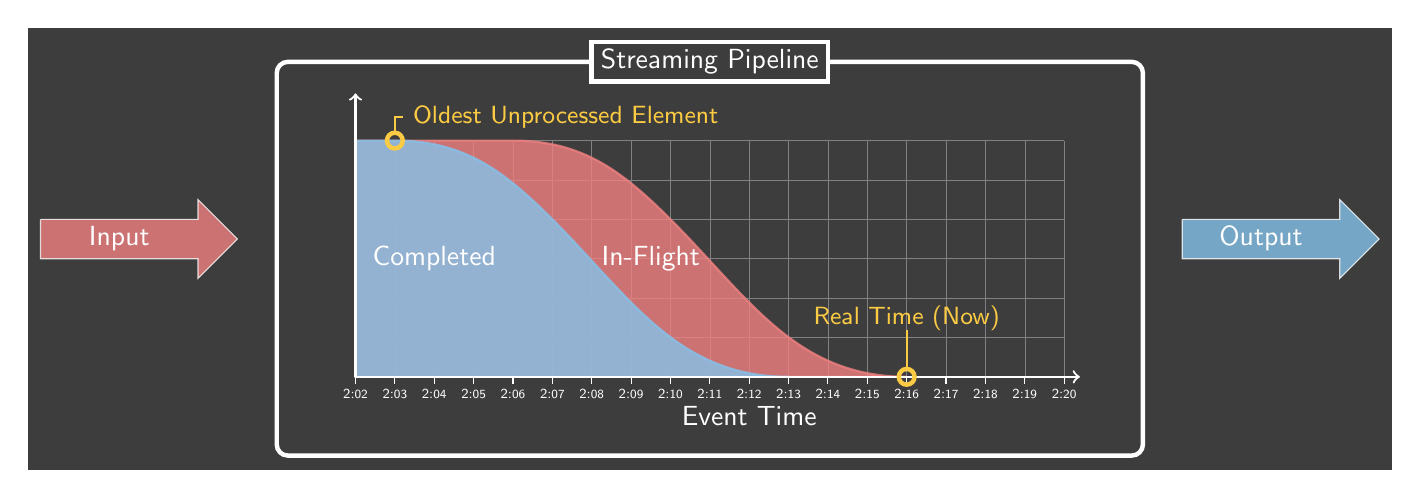
\begin{tikzpicture}
[color=white,show background rectangle, background rectangle/.style={fill=\BackBorder},/tikz/inner frame sep=\BackBorderWidth,font=\sffamily]
	\draw[step=0.5cm,gray,very thin] (1,1) grid (10,4);
	         
	
	\draw [thick, lred, fill=lred, opacity=0.8]
		 (3,4) to [out=0,in=135] 
		 (5,3) to [out=315,in=180] 
		 (8,1) -- (1,1) -- (1,4) -- 
		 (3,  4);
	\draw [thick, lblue, fill=lblue, opacity=0.8]
		 (1.5,4) to [out=0,in=135]
		 (3.5,3) to [out=315,in=180]
		 (6.5,1) -- (1,1) -- (1,4) -- 
		 (1.5, 4 );
	\node at (2,2.5) {Completed};
	\node at (4.75,2.5) {In-Flight};
	         
  
	\draw[thick,->] (1,1) -- (10.2,1);
	\node at (6,0.5) {Event Time};
	\draw[thick,->] (1,1) -- (1,4.6);
	\foreach \x in {1,1.5,2,2.5,3,3.5,4,4.5,5,5.5,6,6.5,7,7.5,8,8.5,9,9.5,10}
		\pgfmathtruncatemacro{\Result}{\x*2}
		\tiny
   		 \draw (\x cm,28pt) -- (\x cm,26pt) node[anchor=north] {2:{\Scale[0.9]{$\z{\Result}$}}};
		 \normalsize
		 
	
	\draw [c_yellow, ultra thick] (1.5,4) circle [radius=0.1];;
	\draw [c_yellow, thick] (1.5, 4.1) -- (1.5, 4.3) -- (1.6, 4.3) node[anchor=west] {\small Oldest Unprocessed Element };
	\draw [c_yellow, ultra thick] (8,1) circle [radius=0.1];;
	\draw [c_yellow, thick] (8, 1.1) -- (8, 1.6);
	\node [c_yellow] at (8, 1.75)  {\small Real Time (Now)};
	
	
	\draw [rounded corners, ultra thick, white] (1,0) -- (11,0) -- (11,5) -- (0, 5) -- (0,0) -- (1, 0);
	\draw [white, ultra thick, fill=c_back_dark] (4, 4.75) -- (7, 4.75) -- (7, 5.25) -- (4, 5.25) -- (4, 4.75) -- (5, 4.75);
	\node at (5.5,5) {Streaming Pipeline};
	
	\draw [fill=lred, opacity=0.8] (-3, 3) -- (-1,3) -- (-1, 3.25) -- (-0.5, 2.75) -- (-1, 2.25) -- ( -1, 2.5) -- (-3, 2.5) -- (-3, 3);
	\draw [fill=lblue, opacity=0.8]   (11.5, 3) -- (13.5,3) -- (13.5, 3.25) -- (14, 2.75) -- (13.5, 2.25) -- ( 13.5, 2.5) -- (11.5, 2.5) -- (11.5, 3);
	\node at (-2, 2.75) {Input};
	\node at (12.5, 2.75) {Output};
	
	
	%\foreach \y in {0,1,2,3,4}
   	%	 \draw (1pt,\y cm) -- (-1pt,\y cm) node[anchor=east] {$\y$};

	
\end{tikzpicture}

\end{document}